\section{Introduction}\label{sec:Intro}

We present a calculator \dots

\subsection{Motivation}

The developments of a Unifying Theory of Programming (UTP)
can involve a number of false starts,
as alphabet variables are chosen
and semantics and healthiness conditions are defined.
Typically, some calculations done just to check that everything
work reveal problems with the theory.
So an iteration occurs by revising the basic definitions,
and attempting the calculations again.
Hopefully, these eventually converge to what becomes a sound and useful
UTP Theory.
In a recent bout of such theory revision and re-calculation,
which required five iterations in total,
the author noted that common patterns of proof-steps kept arising
in each iteration.

We have recently started to explore using UTP
to do the  formal modelling of a language,
called ``Process Modelling Language''
(PML)\cite{DBLP:journals/infsof/AtkinsonWN07}.
%It quickly became apparent that PML and similar (business) process
%notations essentially involve concurrency with global shared mutable state.
%There has been work using UTP
%to model concurrent programs with shared mutable state,
%most notably
%with an encoding into action systems having been done by
%Woodcock and Hughes\cite{DBLP:conf/icfem/WoodcockH02}.
%We have been looking at adapting this work to provide a UTP semantics
%for PML.
%In addition, we have started to take an interest in the ``Views'' paper
%by Dinsdale-Young and colleagues\cite{conf/popl/Dinsdale-YoungBGPY13},
%that provides a framework within which it is possible
%to construct instances of many different concurrency theories,
%ranging from
%type-theory \cite{tal-toplas,Smit00b,journals/fuin/AhmedFM07},
%Owicki-Gries\cite{Owicki76},
%separation logic\cite{conf/lics/CalcagnoOY07}
%and rely-guarantee\cite{Jones83}
%approaches,
%among others.
So we started by taking the action-system UTP semantics for Unifying Theories
of Parallel Programming (UTPP) \cite{DBLP:conf/icfem/WoodcockH02},
and reworking it to use a system for generating unique labels,
in order to give a slight improvement to the compositionality
of the semantics. This we call a Unifying Theory of Concurrent Programming
(UTCP) and details of this are,
at the time of writing,
accepted for publication\cite{conf/tase/BMN16}.

We give a very brief overview here of this theory.
The language assumes atomic actions ($A$) that modify a generic state,
and four composition operators: sequential ($\lseq$), parallel ($\parallel$),
non-deterministic choice ($\pcond$) and non-deterministic iterations ($\piter{}$)
\[
   P ::= A \mid P \pseq P \mid P \parallel P \mid P \pcond P \mid \piter P
\]
Note that this is essentially the same as the baseline ``Command'' language
in the Views paper\cite{conf/popl/Dinsdale-YoungBGPY13}.
In UTCP we have two distinct groups of observations:
\begin{itemize}
  \item
    Variables that track changes during execution
    (dynamic observations),
    modelling the generic state ($s,s'$)
    and the global label-set ($ls,ls'$) used to manage control-flow.
  \item
    Variables that record static parameters such as start ($in$)
    and stop ($out$) labels for a construct,
    as well as a label generator ($g$) associated with each construct.
\end{itemize}
So our UTCP theory is based on a non-homogeneous relation
with alphabet $s$, $s'$, $ls$, $ls'$, $g$, $in$, and $out$.


The theory with its somewhat unusual arrangement of observation variables
did \emph{not} emerge as an immediate and obvious solution.
The theory design started with an homogeneous alphabet with $g'$, $in'$ and $out'$
being present, and the need for the dynamic/static distinction only emerged
through various iterations of the theory.

The first problem was relatively minor
---a lot of the semantics talks about the presence of various
labels in the global label-set, or alternatively, their  absence,
and of modifications to that set.
This resulted in very wide expressions,
so some shorthand notations were introduced.

The second problem was more serious.
It often took long painstaking calculations to discover problems
with a proposed version of the theory,
typically when trying to calculate outcomes associated with
$A \pseq B$and then  $A \parallel B$.
In every case the fault was traced back to sequential composition%
\footnote{
In the author's experience,
when building semantic theories involving concurrency or parallelism,
it is always sequential composition that causes the most difficulty
}
.
The calculations for sequential and parallel composition
required typically about 400 lines of \LaTeX\ and resulted
in 7 full pages of output,
an extract of which is shown in Fig. \ref{fig:attempt4}.

\begin{figure}
  \centering
  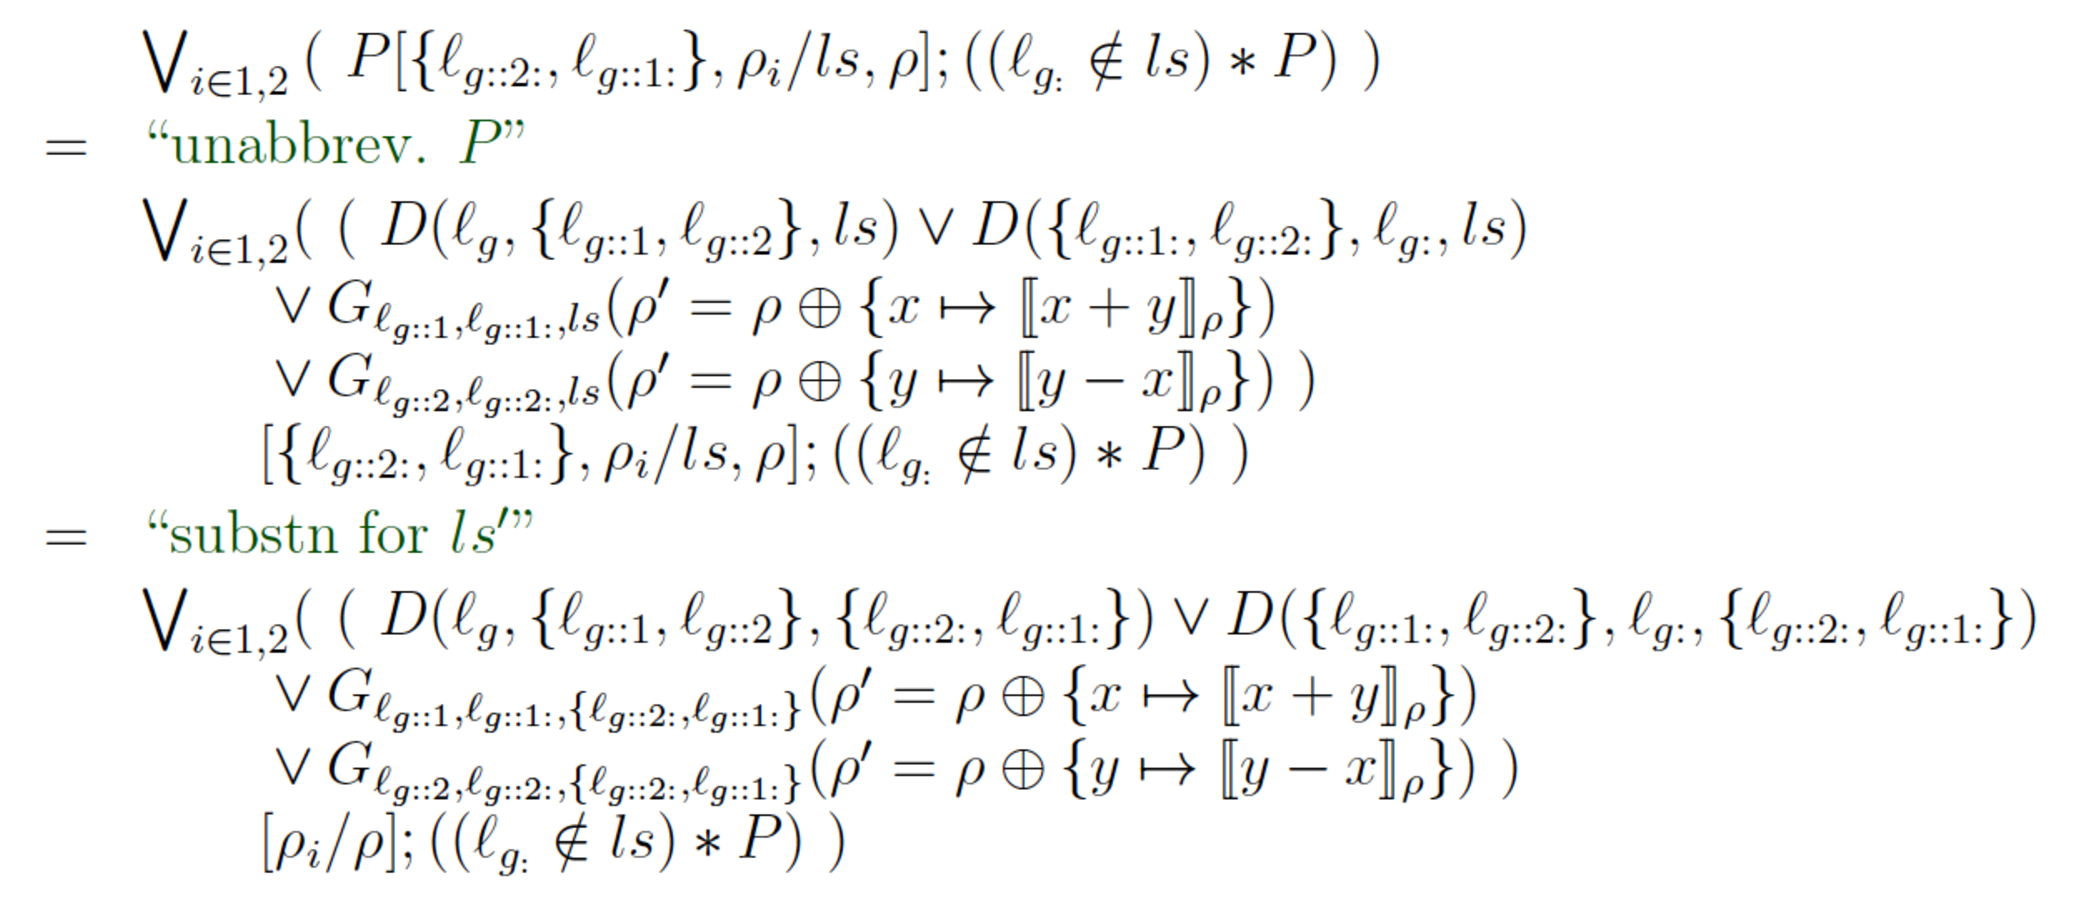
\includegraphics[width=4.5in]{Attempt4.eps}\\
  \caption{Extract from 4th attempt to calculate $x:=x+y \parallel y:=y-x$}
  \label{fig:attempt4}
\end{figure}

With choice and iteration to be covered,
it was becoming very clear that a better way was required
for checking semantic outcomes.

If we consider the reasoning processes used in the development
and deployment of a theory, we can see a spectrum ranging from informal,
through to fully mechanised: hand calculation; simulation; proof assistant;
and automated theorem provers.
The level of detail, complexity, and rigour rises as we proceed along the spectrum.
The calculator described here is designed
to assist with the exploratory hand-calculation phase early on,
by making it easier to calculate, and to manually check the outcomes.
It is not intended to provide the soundness guarantees that are quite rightly
expected from the tools further along the spectrum.


\subsection{Structure of this paper}
